
\documentclass[12pt]{scrartcl}
\usepackage[utf8]{inputenc}
\usepackage{amsmath}
\usepackage{amsfonts}
\usepackage{graphicx}
\usepackage{epstopdf}
\usepackage{soul}
\usepackage{float}
\usepackage{listings}

\title{Information Theory Homework 3}
\author{Sebastian Hörl\\Personal number: 9007126130\\E-Mail: hoerl.sebastian@gmail.com}
\date{\today}

\lstset{ %
  basicstyle=\footnotesize\ttfamily    
}

\begin{document}
\maketitle

The task is to investigate the progression of the entropy in the 1D cellular automaton with rule R174. The transitions can be seen in table \ref{tab:1}.

\begin{table}
\centering
\begin{tabular}{c|c|c|c|c|c|c|c}
111 & 110 & 101 & 100 & 011 & 010 & 001 & 000\\ \hline
1 & 0 & 1 & 0 & 1 & 1 & 1 & 0
\end{tabular}
\caption{Transition table for rule R174}
\label{tab:1}
\end{table}

\subsection*{Reversibility}

At first one can think about an initial pattern, that is 010101... clearly the cellular automaton will, one after another, detect the inputs 010, 101, 010, 101 and so on. All of these substrings will generate a 1, so the resulting state after one iteration will be ``all 1''. Now one can think of the initial state 101010... which will produce the same inputs to the transition function. Again, the output will be ``all 1''. 
The condition for having a reversible CA rule is ``having one unique preceding state for every state that can be generated''. With this simple example one can already see that for ``all 1'' there are already two possible preceding states, so the rule is not completely reversible.

However, when looking at the simulation\footnote{Source code at \texttt{https://github.com/blogsh/it3}} in figure \ref{fig:plot}, using the initial FSA that is given in the task, one can already assume the rule to be ``almost reversible'', because for every time step the only effect of the rule here is a shifting of the state to the left (ignoring the artifacts created through the finite grid and the resulting boundary conditions).

One observation for ``almost reversible'' rules is that the preceeding state can be reconstructed by looking at a subsequence of the current state and the first $2r$ bits of the (position-wise) same sequence in the preceeding state. In this example the surrounding is $r=1$. 

So except for the initial step it is clear that the rule is locally reversible, because it is just a shift to the left. The question that needs to be answered when deciding whether the rule is almost reversible is, whether one can reconstruct the initial state from the second state if one knows the first two bits of the initial one.

The rule works in a way that a zero, encapsulated by two ones is transformed to a one. This is done by the rule $101 \rightarrow 1$ and is the only exception to the shifting dynamics. This rule makes sure that after one iteration there are only blocks of zeros that are at least 2 symbols long.

So irregularities in the generation of the next state can only happen within the first 2 bits. If one knows, that the initial state starts with $01$, $10$ or $11$, one automatically knows how to extend the sequence if the second state was ``all 1''. Therefore, indeed, the rule is almost reversible.

\begin{figure}
\centering
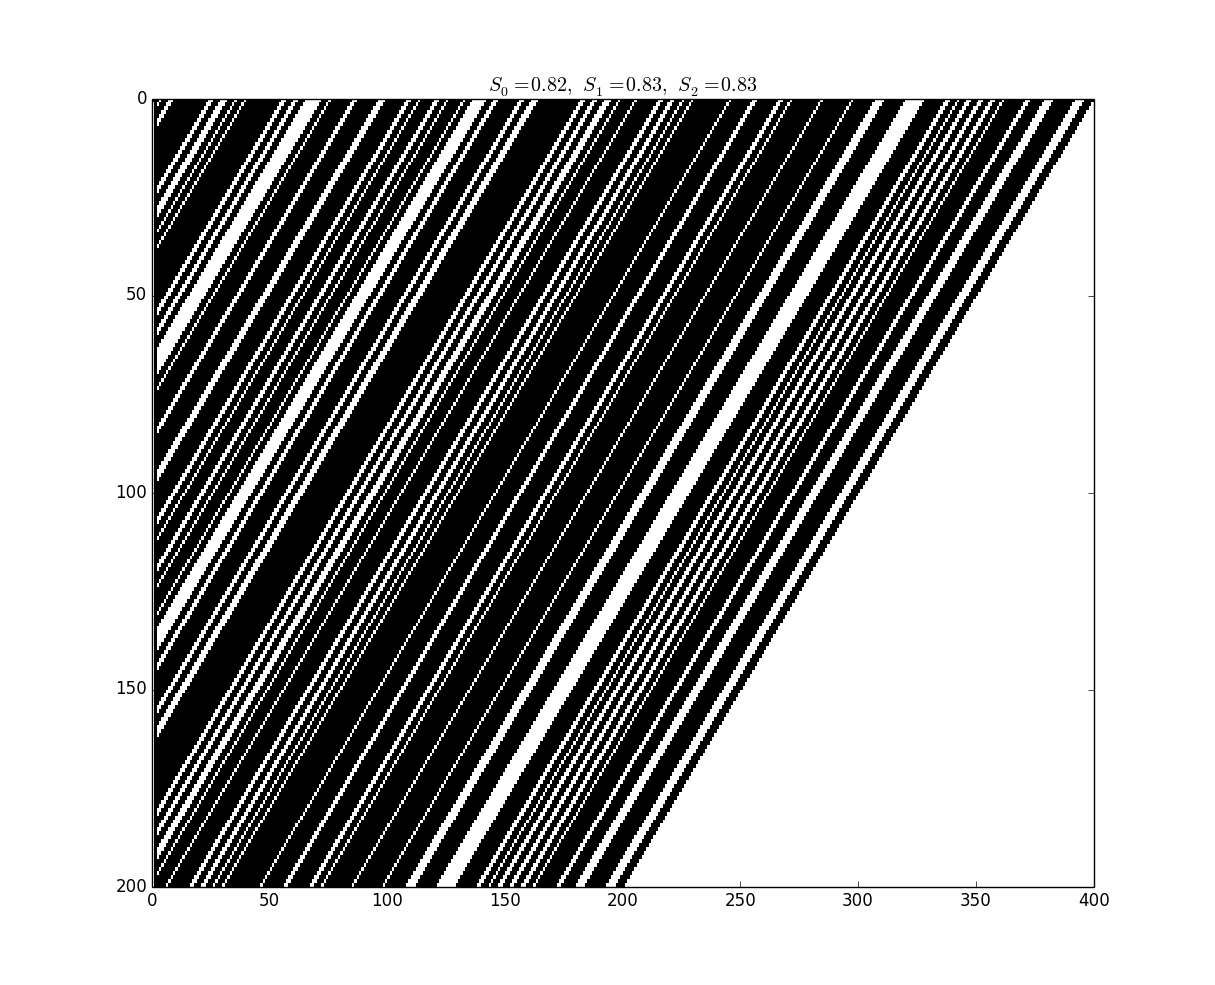
\includegraphics[width=0.8\textwidth]{plot.png}
\caption{Simulation of the CA}
\label{fig:plot}
\end{figure}

\subsection*{Initial Entropy}

The given system can be transformed to the Markov model, that can be seen in figure \ref{fig:b}.

\begin{figure}
\centering
\includegraphics[width=0.3\textwidth]{b.eps}
\caption{Initial Markov Model}
\label{fig:b}
\end{figure}

The output for the HMM would be:

\begin{equation}
f(A) = 1 \ \ \ f(B) = 0 \ \ \ f(C) = 1 \ \ \ f(D) = 1
\end{equation}

The stationary distribution for the states can be determined:

\begin{equation}\begin{aligned}
P(B) &= \frac{1}{2}P(A) + \frac{1}{2}P(B) &\rightarrow P(B) = P(A)\\
P(C) &= \frac{1}{2}P(A) + \frac{1}{2}P(B) &\rightarrow P(C) = P(A)\\
P(D) &= P(C) &\rightarrow P(D) = P(A)
\end{aligned}\end{equation}

Normalizing the distribution gives:

\begin{equation}
P(A) + P(B) + P(C) + P(D) = 4 P(A) = 1 \rightarrow P(A) = \frac{1}{4}
\end{equation}

The distribution for the output is:

\begin{equation}\begin{aligned}
P(0) &= P(B) = \frac{1}{4}\\
P(1) &= P(A) + P(C) + P(D) = \frac{3}{4}
\end{aligned}\end{equation}

Using this distribution the initial entropy can be computed:

\begin{equation}\begin{aligned}
S_0 &= P(0) \log \frac{1}{P(0)} + P(1) \log \frac{1}{P(1)}\\
&= \frac{1}{4} \log 4 + \frac{3}{4} + \log \frac{4}{3}\\
&= 0.81128
\end{aligned}\end{equation}

\subsection*{FSA after one iteration}

At first the previous Markov chain can be modified to be built of pairs. Moving from one pair to another, one can define the output for the next iteration step in terms of the transition function of rule 174 (figure \ref{fig:c1}).

\begin{figure}
\centering
\includegraphics[width=0.5\textwidth]{c1.eps}
\caption{Paired Markvo model with transitions}
\label{fig:c1}
\end{figure}

The result is a new Hidden Markov Model, which can be seen in figure \ref{fig:c2}.

\begin{figure}
\centering
\includegraphics[width=0.3\textwidth]{c2.eps}
\caption{Hidden Markov Model}
\label{fig:c2}
\end{figure}

One can see that the red nodes both with probability $\frac{1}{2}$ generate a transition to the upper right node and with probability $\frac{1}{2}$ to the lower right one. Therefore they are equal and can be combined. The same is true for the blue dots. They both always lead to the lower middle node, generating a 1. After simplifying the HMM, it looks as in figure \ref{fig:c3}.

\begin{figure}[h!]
\centering
\includegraphics[width=0.3\textwidth]{c3.eps}
\caption{Simplified Markov Model}
\label{fig:c3}
\end{figure}

Then again, the circled nodes are equivalent and can be merged, leading to the FSA in figure \ref{fig:c31}.

\begin{figure}[h!]
\centering
\includegraphics[width=0.3\textwidth]{c31.eps}
\caption{FSA after one iteration}
\label{fig:c31}
\end{figure}

So after applying the transition rule one arrives at the exact same FSA as before.

\subsection*{Entropy in subsequent iterations}

Because after one iteration one arrives at the same FSA as before, applying the rule again won't change anything for the calculation of the entropy. Thus one can state the for $t=1$ and $t=2$ that the entropy will be the same es in the initial step. This also corresponds to the result that the rule is almost reversible.	

\begin{equation}
S_2 = S_1 = S_0
\end{equation}

\end{document}

